% Copyright (C) 2026 Johan Roenby
% SPDX-License-Identifier: GPL-3.0-or-later
\documentclass[11pt,a4paper]{article}

\usepackage[margin=2.3cm]{geometry}
\usepackage[T1]{fontenc}
\usepackage{lmodern}
\usepackage{amsmath}
\usepackage{graphicx}
\usepackage{booktabs}
\usepackage{array}
\usepackage{siunitx}
\usepackage{subcaption}
\usepackage{pgfplots}
\usepackage{xcolor}
\usepackage{listings}
\usepackage[hidelinks]{hyperref}

\usepgfplotslibrary{groupplots}
\pgfplotsset{compat=1.17}
\setlength{\emergencystretch}{3em}
\renewcommand{\topfraction}{0.9}
\renewcommand{\bottomfraction}{0.8}
\renewcommand{\textfraction}{0.07}
\renewcommand{\floatpagefraction}{0.75}
\setcounter{totalnumber}{5}
\lstset{basicstyle=\ttfamily\small, columns=fixed, basewidth=0.52em, frame=single, framesep=4pt}

% Numbers from the executed test suite (makeData.py)
\input{generated/results.tex}

% Table rows from a file (the primitive input is expandable, as needed for
% \multicolumn at the start of a row)
\makeatletter
\newcommand{\inputrows}[1]{\@@input #1 }
\makeatother

\newcommand{\sP}{\texttt{surfacePosition}}
\newcommand{\iH}{\texttt{interfaceHeight}}

\title{The \sP{} function object:\\ implementation and tests}
\author{Johan Roenby}
\date{\today}

\begin{document}
\maketitle

\begin{abstract}
\noindent \sP{} is an OpenFOAM function object that reports the height and
position of a volume-of-fluid interface at a set of locations, with the same
entries and output as OpenFOAM's \iH{}, which integrates the interpolated
volume fraction along a sampled line. \sP{} finds the cells crossed by each
line once and follows them through mesh changes by a flood fill, so its cost
per write does not depend on the mesh size, and it sums the lengths of the
line inside the liquid, cutting each interface cell geometrically with the
isosurface of the volume fraction. This report describes the implementation
and the test suite in \texttt{test}. All numbers, tables and figures are
generated from the output of one run of the suite (wall time \suiteTime). In a
\timingCells-cell case on \timingProcs{} processors, \sP{} costs
\SI{\timingSP}{ms} per time step for \timingLines{} lines, against
\SI{\timingIH}{ms} for \iH{}; on the exact stream function wave it is more
accurate than \iH{} on the same mesh, and it is exact for flat interfaces,
also on faces and processor boundaries.
\end{abstract}

% --------------------------------------------------------------------------- %
\section{Usage}

\sP{} is built into the library \texttt{libsurfacePosition} by
\texttt{Allwmake} in its repository. It links OpenFOAM's \texttt{finiteVolume},
\texttt{meshTools}, \texttt{sampling}, \texttt{lagrangian} and
\texttt{geometricVoF} libraries, and is released, like OpenFOAM, under the
GNU General Public License, version 3 or later. It needs OpenFOAM.com
\compatFirst{} or later (section~\ref{sec:compat}). Its entries and output are those of \iH{}, so
that a dictionary of \iH{} works after changing its \texttt{type} and
\texttt{libs}, and post-processing tools for \iH{} read its output:
\begin{lstlisting}
surfacePosition1
{
    type            surfacePosition;
    libs            (surfacePosition);
    locations       ((0 0 0) (10 0 0) (20 0 0));
    alpha           alpha.water;    // default alpha
    liquid          true;           // alpha is the liquid's
    direction       (0 0 -1);       // downwards, default gravity
    mode            accumulated;    // accumulated, highest or lowest
    surfCellTol     1e-8;           // interface cells
    isoFaceTol      1e-8;           // tolerance of the isosurface cut
    checkLineCells  false;          // tests: compare line cells with all cells
    fullSearchInterval 0;           // full search every N mesh changes
}
\end{lstlisting}
The \iH{} entry \texttt{interpolationScheme} is not used. The files
\texttt{height.dat} and \texttt{position.dat} in
\texttt{postProcessing/<name>/<time>} hold, per location, the height $h_B$ of the liquid (in the mode, below) above
the lower boundary, where the line leaves the mesh along the direction, the height
$h_L = h_B - h_{LB}$ of the interface above the location, where $h_{LB}$ is the
height of the location above the lower boundary, and the position of the
interface, the location moved by $h_L$ against the direction. As in \iH{}, a
dry line gives $h_B = 0$, and a line missing the mesh $h_B = 0$ and
$h_L = \mathrm{GREAT}$ ($10^{15}$). The \texttt{mode} sets which height is
reported: \texttt{accumulated} (default), the length of the line in the liquid
as in \iH{}; \texttt{highest}, the top of the highest liquid along the line,
e.g.\ including droplets above the surface; or \texttt{lowest}, the top of the
lowest liquid part, the first transition from liquid to gas going up the line.
The headers of both files state the mode in a comment line
(\texttt{\# Mode : accumulated}), so the columns are unchanged.

% --------------------------------------------------------------------------- %
\section{Implementation}

\subsection{Lines}
Through each location a line runs along the unit downward direction
$\mathbf{t}$ (the \texttt{direction} entry, or gravity), from above the mesh to
below it, across the bounding box of the mesh plus a margin of the box
diagonal for mesh motion, wherever the location is.

\subsection{Cells crossed by a line}
Whether a line $\mathbf{x}(s) = \mathbf{x}_0 + s\,\mathbf{t}$,
$0 \le s \le L$, crosses a convex cell is decided by clipping the parameter
interval against the half-spaces of the cell faces. For a face with outward
area vector $\mathbf{S}_f$ and centre $\mathbf{x}_f$, let
$a = \mathbf{S}_f\cdot\mathbf{t}$ and
$b = \mathbf{S}_f\cdot(\mathbf{x}_f - \mathbf{x}_0)$. For $a > 0$ the
interval is cut above at $s = b/a$ (the line leaves), for $a < 0$ below (the
line enters). The face is taken as parallel to the line if the distance of the
line from the face plane changes by less than a tolerance along the whole
line,
\begin{equation}
  |a|\,L \le \tau, \qquad \tau = 10^{-9}\,|\mathbf{S}_f|^{3/2},
  \label{eq:parallel}
\end{equation}
and the cell is then rejected only if $b < -\tau$. A line lying in a face
plane is thereby inside the cells on both sides. The cell is crossed if the
clipped interval has a length above $10^{-15}L$; its ends $s_\mathrm{in}$ and
$s_\mathrm{out}$, the segment of the line in the cell, are stored with the
cells.

The cells are found once by a \texttt{faceOnlySet} with a cached
\texttt{meshSearch}, plus the cells nearest to five points of the line inside
the local mesh bounds, which catch lines lying on faces. These cells seed the
flood fill below, which completes the set.

\paragraph{Flood fill.}
After a mesh change the cells are found again without a search tree, by a
flood fill that tests the face neighbours of cells crossing the line. The
seeds are the old line cells, mapped through \texttt{reverseCellMap} after a
topology change (\texttt{updateMesh}) and unchanged after mesh motion
(\texttt{movePoints}). If no seed crosses the line any more, rings of face
neighbours around the seeds are tested, up to 10 rings, until a ring holds a
cell crossing the line.

The flood fill and the ring search continue across processor faces: a
candidate cell reaching a processor face sends the cell on the other side to
the neighbouring processor, with the number of rings still to search around
it. All lines are processed together, with one exchange per round, until no
processor has candidates to send. A line that moves into a neighbouring
processor subdomain is thereby followed (section~\ref{sec:moving}). A line
that moves further than the ring limit, or that is connected to its old cells
only through cyclic faces, is only found by a full search, done every
\texttt{fullSearchInterval} mesh changes if requested.

With \texttt{checkLineCells}, the cells found after every mesh change are
compared with all cells of the mesh that cross the line, and the numbers of
missing and extra cells are written to the log. The test suite uses this to
verify the flood fill.

\subsection{Liquid along a line}
At each write, each cell of a line contributes the part of its segment
$[s_\mathrm{in}, s_\mathrm{out}]$ that lies in the liquid:
\begin{itemize}
\item a full cell, $\alpha \ge 1 - \epsilon$ with
  $\epsilon$ = \texttt{surfCellTol}, its whole segment, without any
  computation;
\item an empty cell, $\alpha \le \epsilon$, nothing;
\item an interface cell, $\epsilon < \alpha < 1 - \epsilon$, the part of the
  segment on the liquid side of the isosurface of $\alpha$, interpolated to the
  mesh points, that cuts the volume fraction $\alpha$ from the cell. The
  function object holds its own point values of $\alpha$, interpolated once
  per write, and its own \texttt{surfaceIteratorIso}, whose
  \texttt{vofCutCell} finds the isosurface as in the \texttt{isoAlpha}
  reconstruction (tolerance \texttt{isoFaceTol}, 100 iterations). With the
  centre $\mathbf{c}$ and area vector $\mathbf{n}$ of the isosurface, oriented
  towards the centre of the submerged part of the cell, the liquid is where
  $(\mathbf{x}(s) - \mathbf{c})\cdot\mathbf{n} > 0$; the segment is cut at
  $s = \mathbf{n}\cdot(\mathbf{c} - \mathbf{x}_0)/(\mathbf{n}\cdot\mathbf{t})$.
  A cell that \texttt{vofCutCell} does not cut is counted as full or empty by
  $\alpha \ge 0.5$.
\end{itemize}
The liquid parts of the cells on each processor are merged where they touch,
so that a column of full cells becomes a single part, and gathered on the
master processor.

\subsection{Heights and positions}
Where several cells cover the same part of a line (a line in a face plane, on
an edge, or on a processor or cyclic face), their liquid lengths are
averaged: after every mesh change the ends of the segments of all line cells,
on all processors, divide the line into pieces, each covered by a known
number of cells. The liquid length of the line is
\begin{equation}
  W = \sum_{\text{liquid parts } p}\ \sum_{\text{pieces } j}
      \frac{|p \cap j|}{n_j},
\end{equation}
where $n_j$ is the number of cells covering piece $j$, and the length of the
line in the mesh is the total length of the covered pieces. As in \iH{}, the
height of the liquid above the lower boundary is $h_B = W$ (or the length in
the mesh minus $W$ with \texttt{liquid false}), the lower boundary being the
end of the last covered piece. A sharp interface on a face, as set by
\texttt{setFields}, needs no special treatment, and droplets or bubbles shift
the height only by their volume along the line.

For the modes \texttt{highest} and \texttt{lowest}, the line is divided at the
ends of the pieces and of the liquid parts, and an interval is in the liquid
if at least half of the cells covering it are. The top of the first liquid
interval from above gives the highest point, and the top of the last run of
liquid intervals the top of the lowest liquid part.

% --------------------------------------------------------------------------- %
\section{Test suite}
\label{sec:tests}

The suite (\texttt{test/Allrun}) runs four tests, each with a
summary log and a \texttt{results.json} read by this report:
\begin{center}
\begin{tabular}{lll}
\toprule
Test & What it checks & Processors \\
\midrule
\texttt{waveAccuracy} & accuracy against an exact wave & 1 and 4 \\
\texttt{specialCases} & interfaces and lines on faces, edges, processor and cyclic patches & 1 and 8 \\
\texttt{movingMesh} & line cells after adaptive refinement and mesh motion & 1 and 4 \\
\texttt{largeTiming} & cost in a large case & \timingProcs \\
\bottomrule
\end{tabular}
\end{center}
\texttt{largeTiming} runs on the last \timingProcs{} cores, bound one process
per core with local memory through an Open~MPI rank file, while the other
tests run on the remaining cores. The suite passes if the checks of
\texttt{specialCases} and \texttt{movingMesh} pass; in the run reported here
they \specialPassed{} and \movingPassed{}, respectively.

\paragraph{About \iH{}.}
\iH{} was added to OpenFOAM by the OpenFOAM Foundation in May 2017
(OpenFOAM-6) and has been in OpenFOAM.com since v2006, which added the
optional \texttt{direction} entry. Its algorithm is the same in all
OpenFOAM.com releases from v2006 to v2606: for each location it builds a
\texttt{midPointAndFaceSet} along the mesh diagonal in the direction, which
points downwards (gravity), with a new
\texttt{meshSearch} at every write, integrates the interpolated volume fraction
along it and sums the result over the processors. The only changes are the
writing of the file headers (removed in v2012, restored on the master
processor in v2406) and the documentation (v2512). The OpenFOAM Foundation
corrected its parallel operation in May 2023 (commit \texttt{1d78434bee},
OpenFOAM-11) by skipping sampling segments between two faces; OpenFOAM.com
does not have this correction. The tests use the v2512 version.

\subsection{Accuracy: exact stream function wave}

\texttt{streamFunFoam} sets the fields to an exact stream function wave
(height \SI{0.125}{m}, depth \SI{0.4}{m}, period \SI{2}{s}) in a periodic
flume one wave length long, at every time step, and a coded function object
writes the exact surface elevation at the lines. The flume has a coarse
($38\times8$) and a medium ($95\times20$) mesh. Twelve vertical lines are
placed in four cell columns, at the cell centre, a quarter cell off it and
\SI{2}{\%} of a cell from a face (fig.~\ref{fig:wave}). The elevations are
compared over one period with \waveMediumSamples{} samples, for \sP{} and
for \iH{} with its default \texttt{cellPoint} and with \texttt{cell}
interpolation.

\begin{figure}[!htbp]
  \centering
  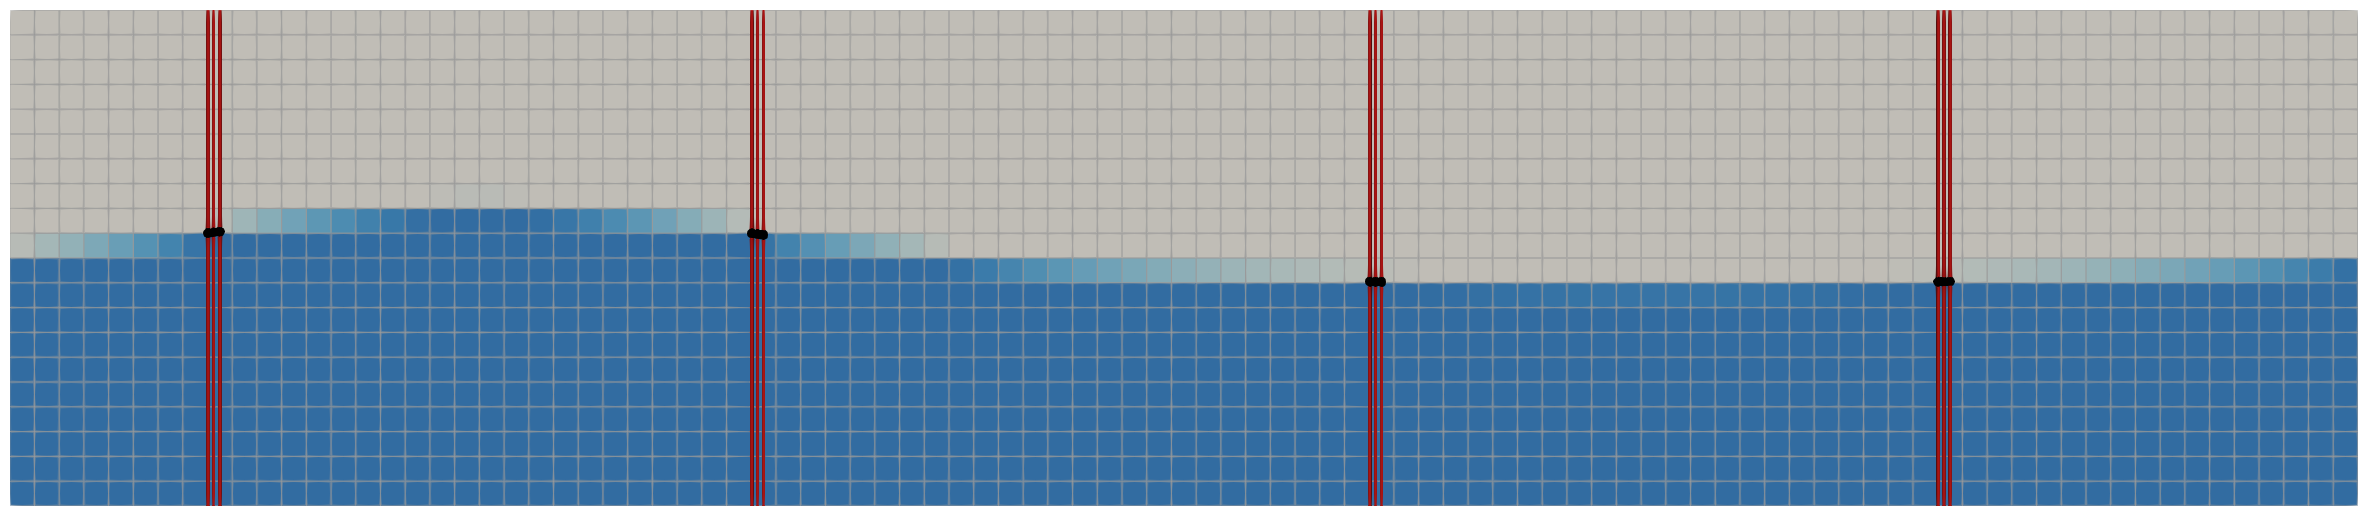
\includegraphics[width=\textwidth]{figures/wave.png}
  \caption{\texttt{waveAccuracy}, medium mesh at $t = \SI{2}{s}$: volume
    fraction (white air, blue water), the \waveMediumLines{} vertical lines
    (red, three per cell column) and the positions found by \sP{}.}
  \label{fig:wave}
\end{figure}

\begin{table}[!htbp]
  \centering
  \caption{Error of the interface elevation against the exact wave [mm]: rms
    per position of the line in the cell (in cell widths from the face), and
    mean and maximum magnitude over all lines and samples.}
  \label{tab:wave}
  \begin{tabular}{lccccc}
    \toprule
    & \multicolumn{3}{c}{rms, line position} & \multicolumn{2}{c}{all lines} \\
    \cmidrule(lr){2-4} \cmidrule(lr){5-6}
    Method & 0.50 & 0.25 & 0.02 & mean & max \\
    \midrule
    \inputrows{generated/tabWave.tex}
    \bottomrule
  \end{tabular}
\end{table}

Table~\ref{tab:wave} shows that \sP{} has the smallest error on both meshes:
\SI{\waveCoarseSPRms}{mm} rms on the coarse mesh against
\SI{\waveCoarseCellPointRms}{mm} for \iH{} (cellPoint), and
\SI{\waveMediumSPRms}{mm} against \SI{\waveMediumCellPointRms}{mm} on the
medium mesh, where its largest error is \SI{\waveMediumSPMax}{mm}. \iH{} with
cell interpolation is biased by a quarter of the cell height
(\SI{\waveCoarseCellMean}{mm} and \SI{\waveMediumCellMean}{mm}); the sign of
this bias follows the direction. Fig.~\ref{fig:waveerror} shows the errors
over the period at a cell centre and \SI{2}{\%} of a cell from a face. The
serial and parallel results \waveParallel.

\begin{figure}[!htbp]
  \centering
  % Error of the elevation over one wave period (waveAccuracy), used by
% report.tex and, as an image for the README, by waveErrorFigure.tex
\begin{tikzpicture}
  \begin{groupplot}[
      group style={group size=2 by 1, horizontal sep=1.6cm},
      width=7.7cm, height=5cm,
      xlabel={$t$ [s]}, xmin=0, xmax=2,
      grid=major, grid style={gray!25},
      legend style={font=\footnotesize}, legend cell align=left,
      tick label style={font=\footnotesize},
    ]
    \nextgroupplot[ylabel={error [mm]},
      title={\footnotesize line \waveLineA, position \waveLineAOffset},
      legend to name=waveLegend, legend columns=3]
    \addplot[blue, thick] table[x=t, y=ihCellPoint] {generated/waveLine\waveLineA.csv};
    \addlegendentry{\iH{}, cellPoint}
    \addplot[red, thick] table[x=t, y=spPlic] {generated/waveLine\waveLineA.csv};
    \addlegendentry{\sP{}, plic}
    \addplot[black!60, dashed] table[x=t, y=spAlpha] {generated/waveLine\waveLineA.csv};
    \addlegendentry{\sP{}, alpha}
    \nextgroupplot[title={\footnotesize line \waveLineB, position \waveLineBOffset}]
    \addplot[blue, thick] table[x=t, y=ihCellPoint] {generated/waveLine\waveLineB.csv};
    \addplot[red, thick] table[x=t, y=spPlic] {generated/waveLine\waveLineB.csv};
    \addplot[black!60, dashed] table[x=t, y=spAlpha] {generated/waveLine\waveLineB.csv};
  \end{groupplot}
\end{tikzpicture}
\\[2pt]
\ref{waveLegend}

  \caption{Error of the elevation over one wave period on the medium mesh, at
    a cell centre and \SI{2}{\%} of a cell width from a face.}
  \label{fig:waveerror}
\end{figure}

\subsection{Special cases}

A closed $10\times10\times10$ cube, cyclic in $x$, decomposed into 8
subdomains, holds a flat interface ($z = 0.537$ inside cells,
$z = 0.5$ on internal and processor faces, $z = 0.3$ on internal faces), a
vertical slab of water ($x < 0.5$), whose interfaces lie on the cyclic and the
processor faces, or two layers of water, below $z = 0.35$ and at
$0.6 < z < 0.75$ with a sharp lower interface. After one short \texttt{interIsoFoam} step, twelve vertical
lines (fig.~\ref{fig:special}) test locations in a cell, on a face plane, on
an edge, on a processor face and edge, on the cyclic patches, on a
cyclic/processor edge and a cyclic/wall edge, far above and far below the
mesh, and outside the domain, with \sP{} in its three modes. The heights and
positions are compared with the exact values: for the flat interfaces
$h_B = z$ in all modes on all lines crossing the mesh; for the slab $h_B = 1$
for $x < 0.5$, 0 for $x > 0.5$, and on the processor faces at $x = 0.5$, where
a full and an empty cell meet, 0.5 accumulated and 1 in the other modes; for
the layers $h_B = 0.5$ accumulated, 0.75 highest and 0.35 lowest; and the
marker of a line missing the mesh for the line outside the domain.

\begin{figure}[!htbp]
  \centering
  \begin{subfigure}{0.49\textwidth}
    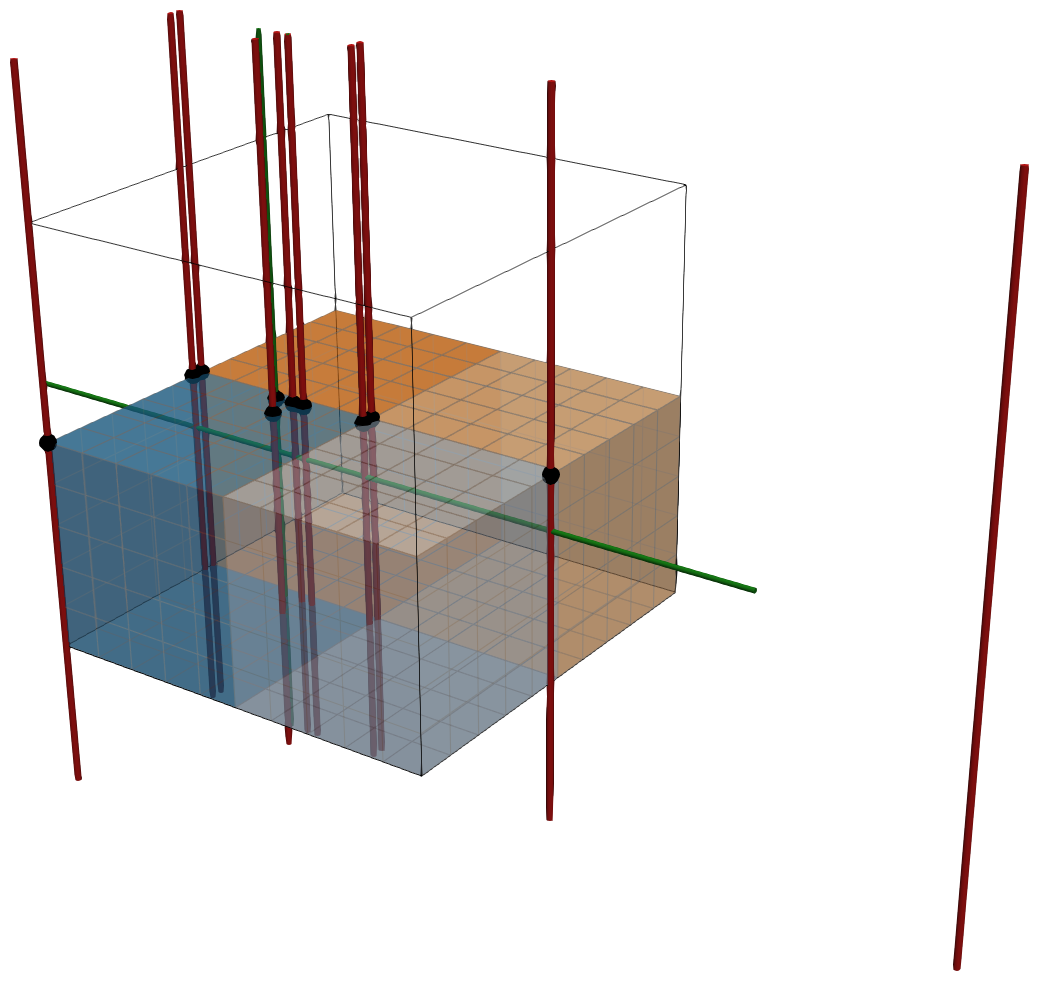
\includegraphics[width=\textwidth]{figures/special_flat500.png}
    \caption{Flat interface at $z = 0.5$}
  \end{subfigure}
  \hfill
  \begin{subfigure}{0.49\textwidth}
    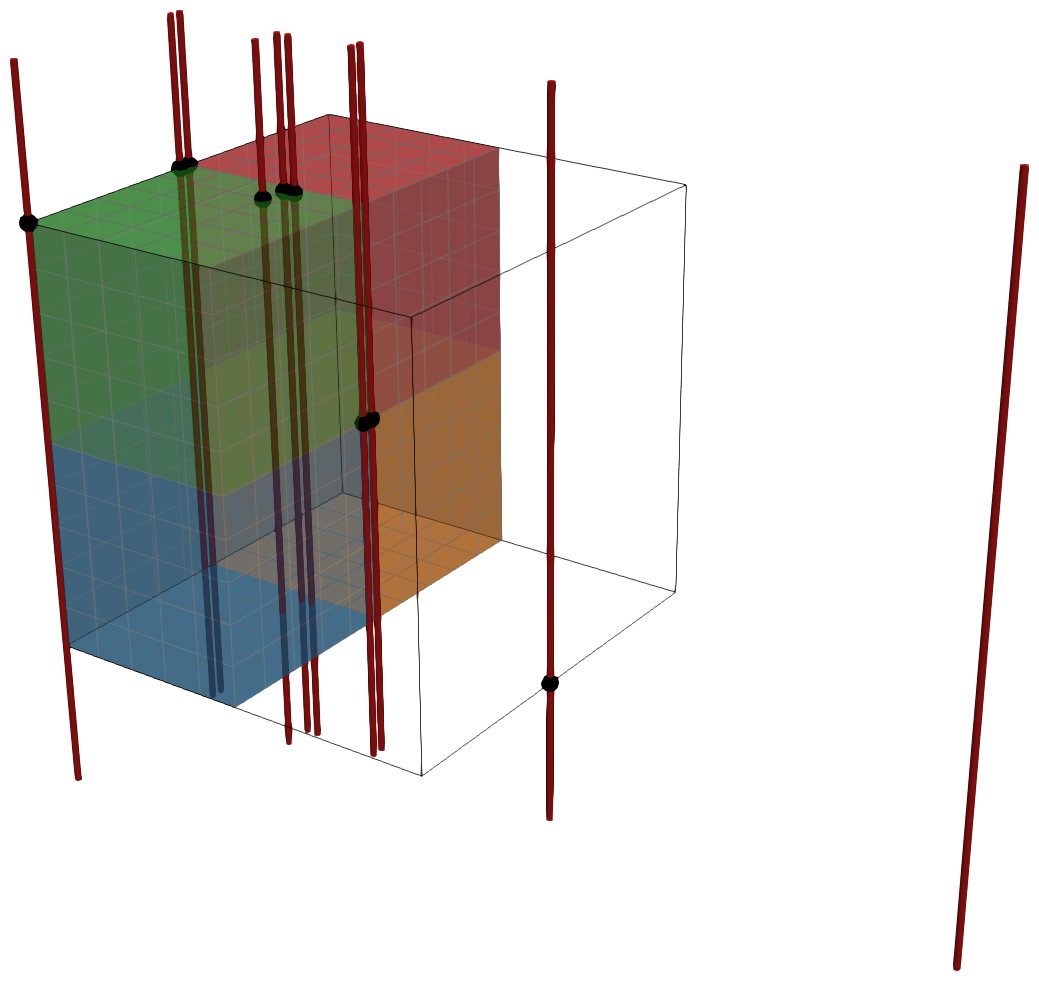
\includegraphics[width=\textwidth]{figures/special_slab.png}
    \caption{Vertical slab of water}
  \end{subfigure}
  \caption{\texttt{specialCases} on 8 processors: water coloured by
    processor, the vertical lines through the locations (red; the line on the
    right is outside the domain) and the positions found by \sP{}.}
  \label{fig:special}
\end{figure}

\begin{table}[!htbp]
  \centering
  \caption{Largest error of the heights $h_B$, $h_L$ and positions of \sP{}
    in its three modes against the exact values [m], over the lines crossing
    the mesh (tolerance \specialTol{}\,m), and the number of lines correctly
    reported as missing the mesh.}
  \label{tab:special}
  \begin{tabular}{llcccc}
    \toprule
    Scenario & Proc. & accumulated & highest & lowest & off mesh \\
    \midrule
    \inputrows{generated/tabSpecial.tex}
    \bottomrule
  \end{tabular}
\end{table}

All heights and positions are exact to round-off in all modes
(table~\ref{tab:special}), in serial and on 8 processors, including the interfaces on processor and cyclic
faces and the lines on faces, edges and patches. Table~\ref{tab:specialIH}
shows $h_B$ of \iH{} on some of the lines. On 8 processors, the lines on
processor faces and edges count the water of the cells on all sides; on the
cyclic patches and their edges it gives 0.5 instead of 1 for the slab; and for
locations far above or below the mesh it gives 0, as its line, of the length
of the mesh diagonal around the location, does not reach the mesh.

\begin{table}[!htbp]
  \centering
  \caption{\iH{}: height $h_B$ [m] above the bottom on some of the special
    lines, for the flat interface at $z = 0.5$ and the slab.}
  \label{tab:specialIH}
  \begin{tabular}{rlcccccc}
    \toprule
    & & \multicolumn{3}{c}{flat, $z = 0.5$} & \multicolumn{3}{c}{slab} \\
    \cmidrule(lr){3-5} \cmidrule(lr){6-8}
    Line & Location & exact & serial & 8 proc. & exact & serial & 8 proc. \\
    \midrule
    \inputrows{generated/tabSpecialIH.tex}
    \bottomrule
  \end{tabular}
\end{table}

\subsection{Moving meshes}
\label{sec:moving}

A 2D standing wave (amplitude \SI{0.05}{m}) in a closed unit box with a
$20\times20$ mesh, one cell thick in $y$, is run with \texttt{interIsoFoam}
in two variants,
in serial and on 4 processors:
\begin{description}
\item[amr] adaptive refinement of the interface cells to two levels at every
  time step with \texttt{dynamicRefineFvMesh}, for \amrSteps{} time steps. The
  refinement also splits the cells in $y$, so that the seven lines, which lie
  in the plane $y = 0$, run in the internal faces of the refined cells
  (fig.~\ref{fig:amr}).
\item[motion] a solid body oscillation of the whole mesh in $x$,
  $\SI{0.05}{m}\,\sin(5.3\,t)$, for \SI{0.6}{s}, with the lines fixed in
  space, so that the line cells change at every time step.
\end{description}

\begin{figure}[!htbp]
  \centering
  \begin{subfigure}[b]{0.36\textwidth}
    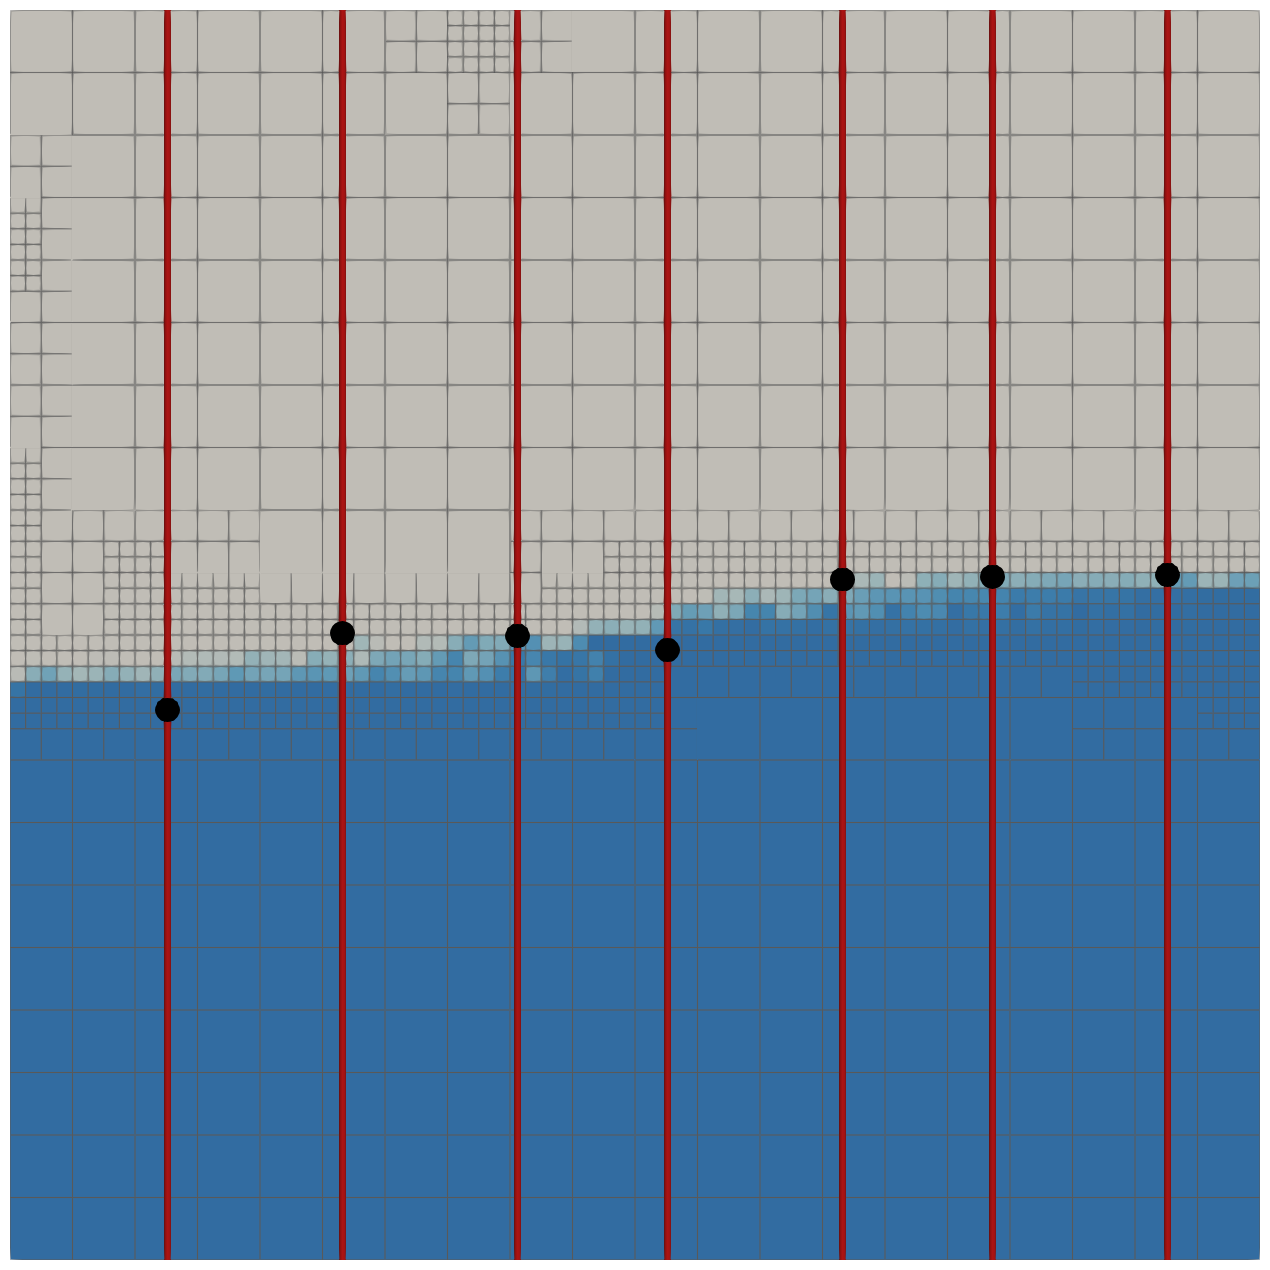
\includegraphics[width=\textwidth]{figures/amr.png}
    \caption{amr, $t = \SI{\amrEndTime}{s}$}
    \label{fig:amr}
  \end{subfigure}
  \hfill
  \begin{subfigure}[b]{0.3\textwidth}
    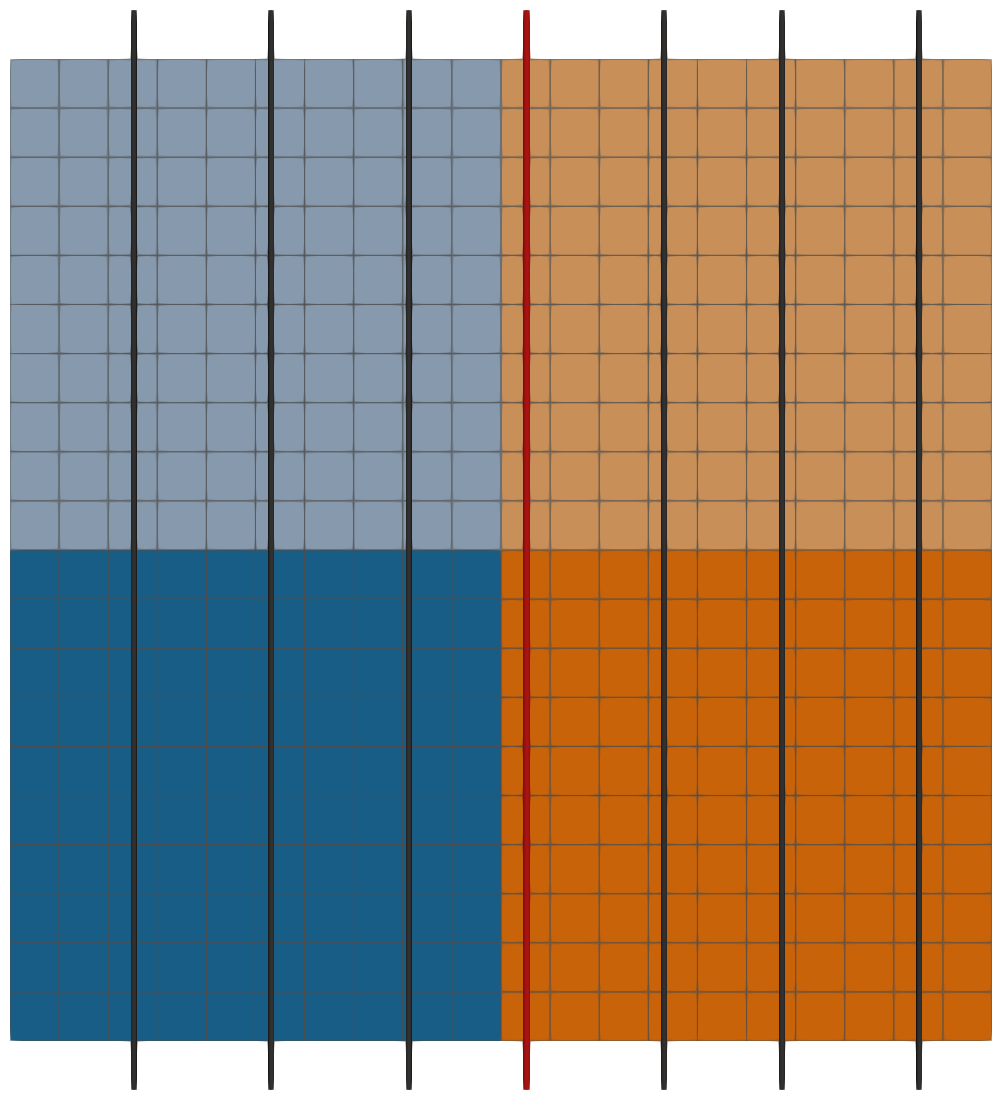
\includegraphics[width=\textwidth]{figures/motion_t0.png}
    \caption{motion, $t = 0$}
  \end{subfigure}
  \hfill
  \begin{subfigure}[b]{0.3\textwidth}
    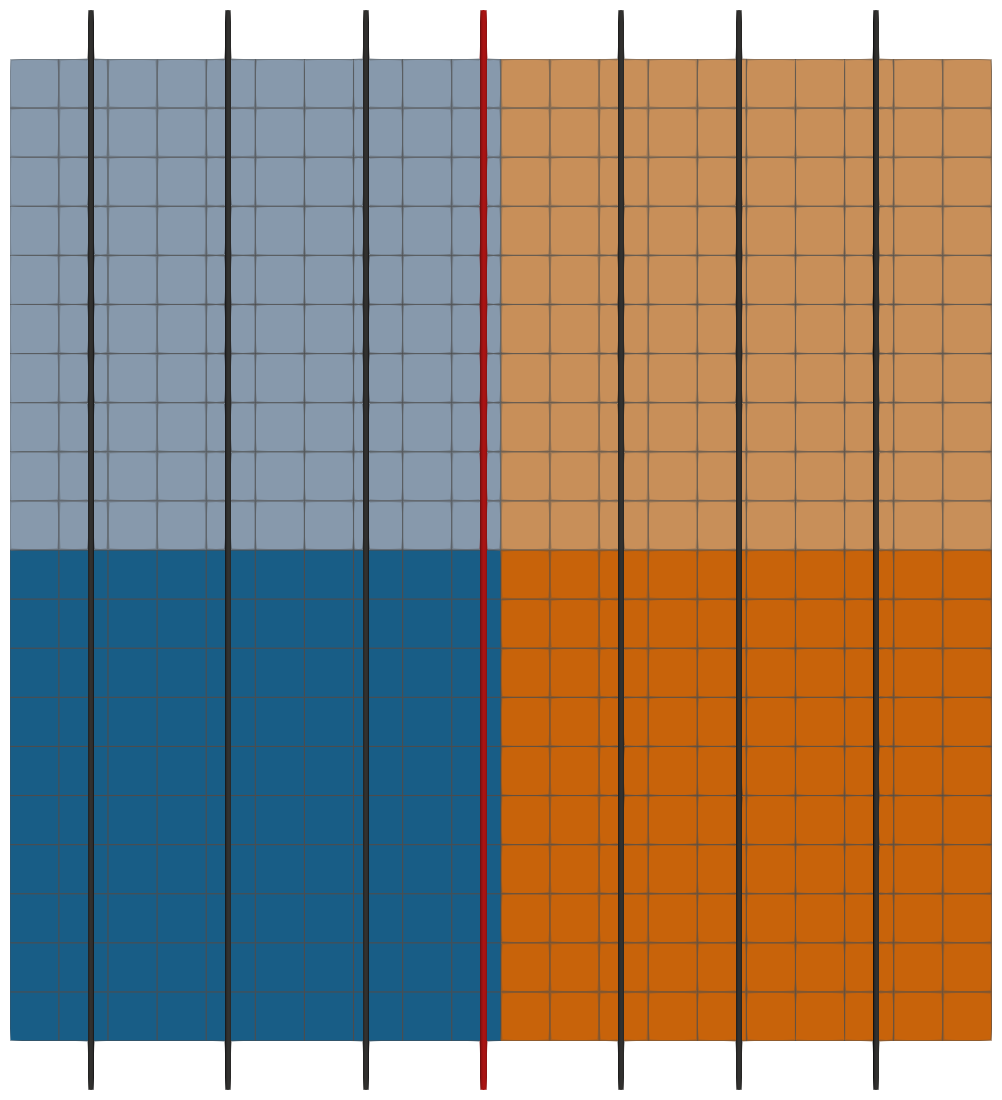
\includegraphics[width=\textwidth]{figures/motion_t2.png}
    \caption{motion, $t = \SI{0.2}{s}$}
  \end{subfigure}
  \caption{\texttt{movingMesh}. (a) Refined mesh, volume fraction, lines and
    the positions found by \sP{}. (b, c) Mesh coloured by
    processor on 4 processors with line 3 (red): the mesh moves right, and
    line 3 passes from the right to the left subdomains.}
  \label{fig:moving}
\end{figure}

\begin{table}[!htbp]
  \centering
  \caption{\texttt{movingMesh}: line cells after all mesh changes compared
    with all cells (\texttt{checkLineCells}), outputs of lines missing the
    mesh (off mesh), and the rms and largest difference of $h_B$ from \iH{} [mm].}
  \label{tab:moving}
  \begin{tabular}{lccccccccc}
    \toprule
    & & & & \multicolumn{3}{c}{line cells} & & \multicolumn{2}{c}{vs.\ \iH{}} \\
    \cmidrule(lr){5-7} \cmidrule(lr){9-10}
    Case & Proc. & Steps & Changes & found & missing & extra & off mesh & rms & max \\
    \midrule
    \inputrows{generated/tabMoving.tex}
    \bottomrule
  \end{tabular}
\end{table}

In all runs the flood fill finds exactly the cells crossing the lines
(table~\ref{tab:moving}): \amrRebuilds{} and \amrParallelRebuilds{} mesh
changes in the serial and parallel amr runs, \motionRebuilds{} in the motion
runs, and no line misses the mesh. In the parallel motion run, line 3 moves
from the subdomains right of a processor boundary to those left of it between
$t = 0.1$ and \SI{0.1125}{s} (fig.~\ref{fig:moving}); the flood fill follows
it across the processor faces and finds all \motionCells{} line cells, as in
serial.

In the amr runs the refinement produces spurious velocities that limit the
time step to about \SI{\amrDeltaT}{s} and throw up droplets. The heights of
\sP{} and \iH{} still differ by at most \SI{\amrMaxDiff}{mm}, since both
measure the liquid volume along the line; serial and parallel amr runs
diverge (\iH{} differs by up to \SI{\amrParallelDiffIH}{mm}). In the motion
runs, serial and parallel flows differ slightly, by up to
\SI{\motionParallelDiffIH}{mm} in \iH{} and \SI{\motionParallelDiffSP}{mm} in
\sP{}.

\subsection{Cost in a large case}

A 3D standing wave in a closed unit cube with \timingCells{} cells is run with
\texttt{\timingSolver} on \timingProcs{} processors (scotch decomposition), with
\timingLines{} vertical lines placed off the cell centres
(fig.~\ref{fig:timing}) and \sP{} and \iH{} writing at every time step. OpenFOAM's profiling gives the time of each function
object and of the flow solution; it is written with the fields after 5
start-up steps and at the end, and the difference gives the time of
\timingSteps{} steps.

\begin{figure}[!htbp]
  \centering
  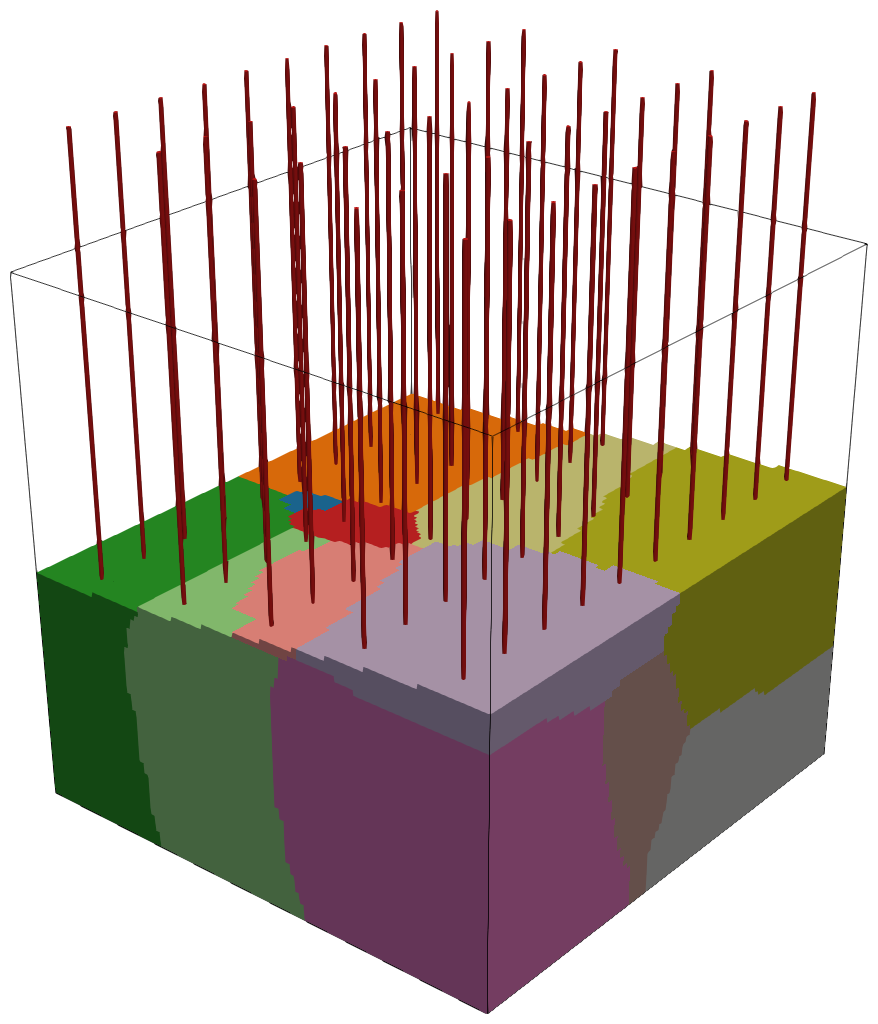
\includegraphics[width=0.4\textwidth]{figures/timing.png}
  \caption{\texttt{largeTiming}: water region coloured by the
    \timingProcs{} processor subdomains, and the \timingLines{} lines.}
  \label{fig:timing}
\end{figure}

\begin{table}[!htbp]
  \centering
  \caption{Time per step (mean over the processors, each including the
    waiting for the others), per line, the range over the processors, and
    the start-up time of the first steps beyond the steady cost (the line
    search), in ms.}
  \label{tab:timing}
  \begin{tabular}{lcccc}
    \toprule
    & per step & per line & range & start-up \\
    \midrule
    \inputrows{generated/tabTiming.tex}
    \bottomrule
  \end{tabular}
\end{table}

\sP{} costs \SI{\timingSP}{ms} per step, \SI{\timingSPFraction}{\%} of the
flow solution, including the interpolation of $\alpha$ to the mesh points,
while \iH{} costs \SI{\timingIH}{ms}, \timingIHFraction{}\,\% of the flow
solution and \timingRatio{} times as much as \sP{}
(table~\ref{tab:timing}). The initial line search of \sP{} takes about
\SI{\timingStartup}{ms} once. The heights of \sP{} and \iH{} agree to
\SI{\timingDiffMax}{mm} (rms \SI{\timingDiffRms}{mm}).

\subsection{Compatibility with OpenFOAM versions}
\label{sec:compat}

\texttt{test/compatibility/Allrun} (not part of \texttt{test/Allrun}) builds
\sP{} with each installed OpenFOAM.com version that has
\texttt{geometricVoF} (\compatOldest{} to \compatNewest{} here) and, where it
compiles and the version runs in parallel, runs the \texttt{specialCases} and
\texttt{movingMesh} tests with that library. Table~\ref{tab:compat} shows the
result of its run on \compatDate. \sP{} compiles and passes these tests with
\compatFirst{} to \compatLast{}. The older versions differ in their
application programming interface: \compatObstacles. With v2306 and v2312,
\sP{} compiles, but \texttt{Pstream::listGatherValues} there only gathers
contiguous types, and the gathering of the liquid parts aborts at the first
write. These are small differences, which could be bridged (with
\texttt{append}, \texttt{last} and \texttt{remove}, an explicit
communication type, a gather with \texttt{PstreamBuffers}, and the
\texttt{fileFormats} include); this was not tried. The installations of
\compatSerialOnly{} were built with an Open MPI that is no longer on this
machine, and run only in serial.

\begin{table}[!htbp]
  \centering
  \caption{Compatibility of \sP{} with the installed OpenFOAM.com versions:
    whether the installation runs, whether \sP{} compiles, the tests with
    it, and the reasons for failures.}
  \label{tab:compat}
  \small
  \begin{tabular}{llccc>{\raggedright\arraybackslash}p{0.33\textwidth}}
    \toprule
    Version & Installation & Compiles & \texttt{specialCases} & \texttt{movingMesh} & Reason \\
    \midrule
    \inputrows{generated/tabCompat.tex}
    \bottomrule
  \end{tabular}
\end{table}

% --------------------------------------------------------------------------- %
\section{Findings of the tests}

Two defects in the line cells of \sP{} were found by the moving mesh tests
and fixed:
\begin{enumerate}
\item \emph{Round-off in the test for faces parallel to the line}
  (\texttt{crossesLine}). A face was taken as parallel to the line only if
  $|a| \le 10^{-300}|\mathbf{S}_f|$. For the lines in the face planes $y = 0$
  of the refined cells, round-off gave $|a|/|\mathbf{S}_f| \approx 10^{-17}$,
  so $b/a$ became an arbitrary distance that could clip a crossed cell away
  and disconnect the flood fill. In a separate run of the serial amr case with
  the old test, all of its \amrRebuilds{} mesh changes missed line cells; with
  eq.~\eqref{eq:parallel} none does.
\item \emph{Lines lost across processor boundaries.} The flood fill followed
  internal faces only. When the motion moved line 3 into the neighbouring
  subdomains, neither side found any cell, and the line was lost for the rest
  of the run. The flood fill now continues across processor faces.
\end{enumerate}
The checks of the suite were tightened accordingly: lines missing the mesh
fail the moving mesh test, and the check scripts' exit codes are passed on to
\texttt{Allrun}.

Earlier versions of \sP{} reported the crossing of the line with the
interface plane of one interface cell, the one with $\alpha$ closest to 0.5.
In the amr runs, droplets with $\alpha$ near 0.5 and steep planes then gave
positions up to metres outside the domain; the liquid length of section 2.4
removes this. The area vector of the isosurface from
\texttt{surfaceIteratorIso}, documented to point from high to low values, gave
the liquid on the wrong side in the flat test, so the liquid side is taken
from the centre of the submerged part of the cell instead.

The tests also show that \iH{} (v2512) is wrong on processor faces and edges,
on cyclic patches, and for locations outside the vertical extent of the mesh
(table~\ref{tab:specialIH}). The first may be what the OpenFOAM Foundation's
parallel correction addresses (section~\ref{sec:tests}); this was not tested.

% --------------------------------------------------------------------------- %
\section{Reproducing this report}

With OpenFOAM v2512 sourced, in the repository of \sP{}:
\begin{lstlisting}
./Allwmake            # libsurfacePosition
cd test
./Allrun              # the test suite, results.json per test
cd report
./Allrun              # makeData.py, makeFigures.py (pvbatch), latexmk
                      # (after ../compatibility/Allrun for section 3.5)
\end{lstlisting}
\texttt{makeData.py} writes the numbers and tables in \texttt{generated/}
from the \texttt{results.json} files and the \texttt{postProcessing} data of
the cases; \texttt{makeFigures.py} renders the figures from the case data with
ParaView. This report was generated from the run of \testRun.

\end{document}
